\chapter{Конструкторский раздел}

Для реализации алгоритма обратной трассировки необходимо рассмотреть алгоритм поиска отраженного луча, вычислений нормалей к сфере и треугольнику, алгоритмы определения пересечения луча и сферы, луча и треугольника.

\section{Поиск отраженного луча}

При пересечении падающего луча с поверхностью необходимо найти направление отраженного луча (если объект не поглощает падающие лучи полностью). Падающий и отраженный лучи, а также нормаль к поверхности в точке касания лежат в одной плоскости (рисунок \ref{rays}), если объект является идеальным зеркалом, то угол падения равен углу отражения.

\begin{figure}[H]
	\begin{center}
		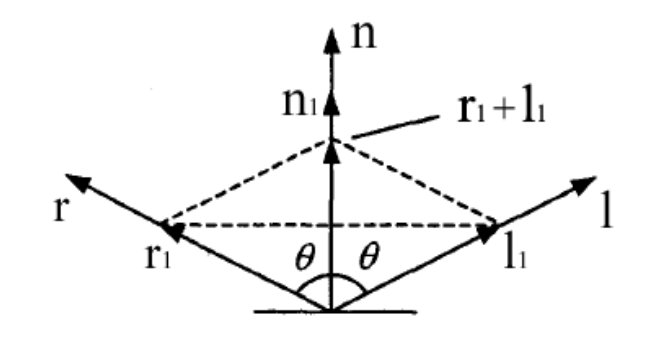
\includegraphics[scale=0.4]{assets/rays.png}
	\end{center}
	\caption{Отражение луча от поверхности}
	\label{rays}
\end{figure}

На рисунке \ref{rays} представлены радиус-векторы от точки касания. $\vec{l}$ направлен на источник света, $\vec{n}$ -- нормаль. Нужно найти вектор отраженного луча $\vec{r}$.

Используем для рассмотрения единичные вектора $\vec{r_1}$ и $\vec{l_1}$, справедливо записать следующее:
\begin{equation}
	\vec{r_1} + \vec{l_1} = \vec{n'},
\end{equation}
где $\vec{n'}$ -- вектор, соответствующий диагонали ромба и совпадающий по направлению с нормалью. Длина этого вектора равна $2cos\theta$.

Так как $\vec{n'}$ по направлению совпадает с $\vec{n_1}$, можно записать следующее:
\begin{equation}\label{many_eq}
	\vec{n'} = 2cos\theta \cdot \vec{n_1} = \vec{r_1} + \vec{l_1}.
\end{equation}

Из (\ref{many_eq}) можно найти единичный вектор отраженного луча:
\begin{equation}\label{rrr}
	\vec{r_1} = 2cos\theta \cdot \vec{n_1} - \vec{l_1} = 2cos\theta \cdot \frac{\vec{n}}{|\vec{n}|} - \frac{\vec{l}}{|\vec{l}|}.
\end{equation}

Используя скалярное произведение векторов $\vec{n}$ и $\vec{l}$ нетрудно найти $cos\theta$:
\begin{equation}
	cos\theta = \frac{(\vec{l}, \vec{n})}{|\vec{l}| \cdot |\vec{n}|}.
\end{equation}

Подставим это значение в (\ref{rrr}):
\begin{equation}
	\vec{r_1} = 2 \cdot \frac{\vec{n} \cdot (\vec{l}, \vec{n})}{|\vec{l}| \cdot |\vec{n}^2|} - \frac{\vec{l}}{|\vec{l}|}.
\end{equation}

Положим, что $\vec{n}$ и $\vec{l}$ нормализованы. Таким образом получим:
\begin{equation}
	\vec{r} = 2\vec{n} \cdot (\vec{l}, \vec{n}) - \vec{l}.
\end{equation}

\section{Вычисление нормалей}

В алгоритме обратной трассировки для поиска отраженного луча вычисляются нормали к объектам. Рассмотрим для используемых в работе полигонов (треугольников) и сферы.

\subsection{Вычисление нормали к полигону (треугольнику)}

Чтобы найти нормаль к плоскости, которую можно задать двумя векторами, достаточно найти векторное произведение. Можно посчитать нормально только один раз, при инициализации сцены, т.к. в каждой точке треугольника нормали совпадают.

Пусть задан треугольник $ABC$, координаты его вершин известны. Нетрудно вычислить координаты векторов $\vec{AB}$ и $\vec{AC}$:
\begin{equation}
	\vec{AB} = \{X_B - X_A, Y_B - Y_A, Z_B - Z_A\}, \vec{AC} = \{X_C - X_A, Y_C - Y_A, Z_C - Z_A\}.
\end{equation}

Векторным произведением будет:
\begin{equation}
	\vec{n} = \vec{AB} \times \vec{AC}.
\end{equation}

Так как мы рассматриваем треугольник как исходную плоскость, необходимо нормализовать нормаль. Тогда координаты вектора нормали вычисляются следующим способом:
\begin{eqnarray}
	X_n = Y_{AB}Z_{AC} - Y_{AC}Z_{AB}, \\
	Y_n = X_{AB}Z_{AC} - X_{AC}Z_{AB}, \\
	Z_n = X_{AB}Y_{AC} - X_{AC}Y_{AB}.
\end{eqnarray}

\subsection{Вычисление нормали к сфере}

Для вычисления нормали к сфере в заданной точке необходимо вычесть координаты центра сферы из координат точки поиска:
\begin{equation}
	n = \{p_x - o_x, p_y - o_y, p_z - o_z\},
\end{equation}
где $\vec{n}$ -- вектор нормали, $p$ -- точка, к которой ищется нормаль, $o$ -- центр сферы. Нормализовать данный вектор можно поделив каждую из координат на радиус сферы.

\section{Поиск пересечения с объектами}

Положение луча в пространстве спустя некое время $t$ можно описать следующим уравнением:
\begin{equation}\label{r_o_d_t}
	\vec{r} = o + \vec{d} \cdot t,
\end{equation}
где $o$ -- начальная точка луча, $\vec{d}$ -- единичный вектор, задающий направление. Можно записать это в другом виде:
\begin{eqnarray}
	x(t) = x_0 + tx_d, \\
	y(t) = y_0 + ty_d, \\
	z(t) = z_0 + tz_d.
\end{eqnarray}

\subsection{Поиск пересечения со сферой}

Сфера задается уравнением вида:
\begin{equation}
	(x - x_c)^2 + (y - y_c)^2 + (z - z_c)^2 = r^2,
\end{equation}
где $c$ -- центр сферы. Вместо $(x, y, z)$ выполним подстановку уравнений луча:
\begin{equation}
	(x_0 + tx_d - x_c)^2 + (y_0 + ty_d - y_c)^2 + (z_0 + tz_d - z_c)^2 = r^2.
\end{equation}

После раскрытия скобок и ряда преобразований получается квадратное уравнение:
\begin{equation}
	At^2 + Bt + C = 0,
\end{equation}
где коэффициенты $A$, $B$ и $C$ принимают значения:
\begin{eqnarray}
	A = x_d^2 + y_d^2 + z_d^2,\\
	B = 2(x_d(x_0 - x_c) + y_d(y_0 - y_c) + z_d(z_0 - z_c)),\\
	C = (x_0 - x_c)^2 + (y_0 - y_c)^2 + (z_0 - z_c)^2 - r^2.
\end{eqnarray}

Коэффициент $A = 1$, так как вектор $\vec{d}$ является единичным.

Если дискриминант уравнения меньше нуля, то луч не пересекает сферу, иначе наименьший положительный корень будет расстоянием от центра сферы до точки пересечения.

При обнаружении двух пересечений, программа будет выбирать ближайшее к наблюдателю. Таковое определяется путем сравнения параметров $t$. Ближней точке пересечения соответствует меньший параметр.

Если одно или оба значения получились отрицательными, это говорит о том, что точка пересечения лежит <<сзади>> относительно начала луча. Такие точки отбрасываются при построении, так как не принадлежат картинной плоскости.

\subsection{Поиск пересечения с треугольником}

Для поиска пересечения используется алгоритм Моллера-Трумбора \cite{trumbor}, работающий оптимально по скорости и по сей день.

Данный алгоритм использует параметризацию точки пересечения $P$ с помощью барицентрических координат:
\begin{equation}
	P = w\vec{A} + u\vec{B} + v\vec{C}.
\end{equation}
Из равенства (\ref{eq}) можно вывести следующие уравнения:
\begin{equation}\label{eq}
	w = 1 - u - v,
\end{equation}

\begin{eqnarray}
	P = (1 - u - v)\vec{A} + u\vec{B} + v\vec{C},\\
	P = \vec{A} + u(\vec{B} - \vec{A}) + v(\vec{C} - \vec{A}),
\end{eqnarray}
где $(\vec{B} - \vec{A})$ и $(\vec{C} - \vec{A})$ являются сторонами треугольника  $ABC$. Последнее равенство можно преобразовать, заменив левую часть на уравнение (\ref{r_o_d_t}):
\begin{equation}
	o + t\vec{d}o - \vec{A} = \vec{A} + u(\vec{B} - \vec{A}) + v(\vec{C} - \vec{A}) - t\vec{d} + u(\vec{B} - \vec{A}) + v(\vec{C} - \vec{A}).
\end{equation}
Перепишем полученное уравнение в более удобной форме:
\begin{equation}
	[-\vec{d}(\vec{B} - \vec{A})(\vec{C} - \vec{A})]\begin{bmatrix}
	t\\ u\\ v
	\end{bmatrix} = o - \vec{A}.
\end{equation}

Можно выразить положение $P$ в пространстве $t, u, v$, где $t$ указывает расстояние от точки пересечения до начала луча и параллельно оси $t$. Если $P$ лежит в треугольнике, то $0 \leq u, v \leq 1, u + v \leq 1$.

Применив метод Крамера, получим:
\begin{equation}
	\begin{bmatrix}
		t\\ u\\ v
	\end{bmatrix} = \frac{1}{[|-\vec{d} \vec{e_1} \vec{e_2}|]} 
	\begin{bmatrix}
		|\vec{T} & \vec{e_1} & \vec{e_2}|\\
		|-\vec{d} & \vec{T} & \vec{e_2}|\\
		|-\vec{d} & \vec{e_1} & \vec{T}|
	\end{bmatrix},
\end{equation}
где $\vec{T} = o - \vec{A}, \vec{e_1} = \vec{B} - \vec{A}, \vec{e_2} = \vec{C} - \vec{A}$. Проведя преобразования, можно записать в следующем виде:
\begin{equation}\label{res_t}
	\begin{bmatrix}
	t\\ u\\ v
	\end{bmatrix} = \frac{1}{\vec{P} \cdot \vec{e_1}}
	\begin{bmatrix}
		\vec{Q} \cdot \vec{e_2}\\
		\vec{P} \cdot \vec{T}\\
		\vec{Q} \cdot \vec{d}
	\end{bmatrix},
\end{equation}
где $\vec{P} = (\vec{d} \times \vec{e_2}), \vec{Q} = (\vec{T} \times \vec{e_1})$. Из (\ref{res_t}) может быть получено необходимое значение $t$.

\section{Алгоритм обратной трассировки}

На входе алгоритма имеется положение наблюдателя, направление его взгляда, угол обзора, описание сцены (присутствующие объекты и их характеристики), описание источника света. Изображение формируется трассировкой лучей через каждый пиксель изображения и установкой возвращаемого лучом цвета.

Для расчета цвета необходимо найти ближайшую точку пересечения с объектом сцены, вычислить нормаль к нему в данной точке и рассчитать интенсивность по формуле (\ref{intensity}). В случае зеркальной поверхности луч отражается и яркость, возвращаемся отраженным лучом, суммируется с яркостью в данной точке.

Для каждого пикселя задается луч \textit{ray} из камеры, и цвет пикселя вычисляется с помощью функции \textit{trace(ray)}. Рассмотрим этапы ее выполнения.
\begin{enumerate}
	\item Поиск точки ближайшего пересечения луча с объектом сцены.
	\item Если такая точка существует, то вызывается функция \textit{shade(point, normal)}, где \textit{point} -- точка пересечения, \textit{normal} -- нормаль к поверхности в данной точке. Иначе цвет пикселя = цвет фона и переход к следующему пикселю.
\end{enumerate}

Рассмотрим этапы выполнения функции \textit{shade(point, normal)}. Изначально цвет пикселя = (0, 0, 0) и осуществляется следующий расчет для каждого источника света.
\begin{enumerate}
	\item Испустить теневой луч из точки пересечения к источнику света.
	\item Если луч не пересекает объект сцены, то цвет = цвет * прямое освещение от источника.
	\item Если поверхность пересечения зеркальная, то если поверхность не является идеальным зеркалом, то внести произвольное отклонение в отраженный луч, тогда цвет = цвет + \textit{trace(отраженный луч)}.
\end{enumerate}

Чтобы выполнение алгоритма занимало меньше времени, можно использовать потоки для параллельности вычислений. Каждый поток может обрабатывать горизонтальную полосу, толщина которой в пикселях определяется количеством потоков:
\begin{equation}
	w = height/ n\_threads,
\end{equation} 
где $height$ -- высота изображения в пикселях, $n\_threads$ -- количество потоков.

\section{Структуры данных}

Рассмотрим необходимые структуры данных. Для хранения геометрических объектов сцены будет использован динамический массив, так как количество элементов не велико, а перебор всех объектов будет достаточно частой операцией.

Для хранения сферы необходимы координаты центра и радиус. Остальные геометрические объекты будут храниться в виде массива полигонов, описываемых тремя вершинами. Для оптимизации вычислений можно также хранить нормаль к полигонам.

Об объектах также необходимо хранить цвет в формате RGB-тройки и характеристики материала, от которых зависит размытость изображения.

\section{Вывод из раздела}

В данном были описаны необходимые алгоритмы и математические основы для их выполнения, а также выбраны необходимые структуры данных.